\subsection{Adjustable Negative Voltage Regulator:}

\begin{tasks}
\task LM337 circuit with variable resistor in his lower value:
\begin{figure}[H]
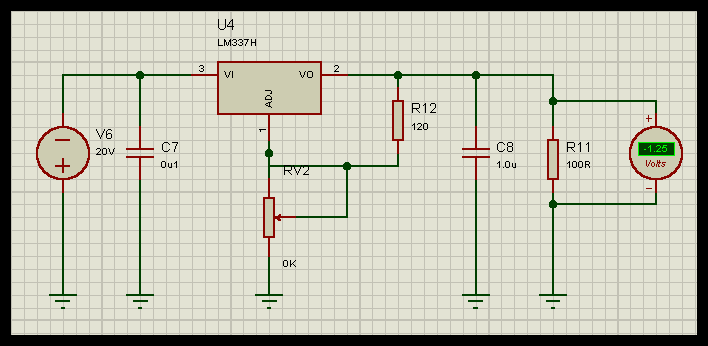
\includegraphics[scale=.6]{min2.png}
\centering \linebreak \linebreak Figure 4.5.0: 0K resistor in adjustable negative voltage regulator circuit.
\end{figure}

\begin{ceqn}
\begin{align}
V_{0_{min}} = -1.25 V
\end{align}
\end{ceqn}

\task LM337 circuit with variable resistor in his maximum value:
\begin{figure}[H]
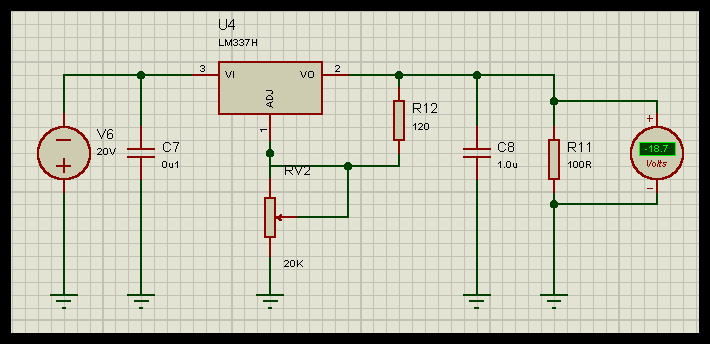
\includegraphics[scale=.6]{max2.png}
\centering \linebreak \linebreak Figure 4.5.1: 10K resistor in adjustable negative voltage regulator circuit.
\end{figure}

\begin{ceqn}
\begin{align}
V_{0_{max}} = -18.7 V
\end{align}
\end{ceqn}
\end{tasks}

\pagebreak